\documentclass[a4paper,12pt]{article}


% add more packages if necessary
\usepackage{xspace}
%\usepackage{graphicx}
%\usepackage{xcolor}
%\usepackage{hyperref}
\usepackage{amsmath}


% TODO: Add your group name
\newcommand{\groupname}{jcd\_dumplings\xspace}


\title{
Project Report \\ 
Group \groupname \\
\vspace{5mm}
\large Java and C\# in depth, Spring 2013
}
\author{
% TODO: Add your names here
Elmer Lukas \\
Nussbaumer Ivo
}
\date{\today}



\begin{document}
\maketitle

\section{Introduction}

This document describes the design and implementation of the \emph{Personal Virtual File System} of group \emph{\groupname}. The project is part of the course \emph{Java and C\# in depth} at ETH Zurich. The following sections describe each project phase, listing the requirements that were implemented and the design decisions taken. The last section describes a use case of using the \emph{Personal Virtual File System}.

% PART I: VFS CORE
% --------------------------------------

\section{VFS Core}

\documentclass[JCDReport.tex]{subfiles} 
\begin{document}


% Give a short description (1-2 paragraphs) of what VFS Core is.
The VFSBase is the base of the file system. It implements the functionality to creating, renaming, deleting, importing, exporting, files and folders. It also provides functionality to query disk information like free space or occupied space. To store the files, there are several compression and encryption options available. Additionally, it creates a new version for every action on the file system, and thus provides a history for the file system. The file system also handles big data by storing all the things on the disk instead of storing them in the RAM before writing it to the disk.

\subsection{Requirements}


% Describe which requirements (and possibly bonus requirements) you have implemented in this part. Give a quick description (1-2 sentences) of each requirement. List the software elements (classes and or functions) that are mainly involved in implementing each requirement.

\subsubsection{Introduction: About the FileSystem and the FileSystemTextManipulator}
Most of the features discussed in this section are about the FileSystem and the FileSystemTextManipulator. The first question might be: the FileSystem and the FileSystemTextManipulator are very similar and provide nearly the same interface, why are the separate? The answer to this question is: separation of concerns and encapsulation.\\
The FileSystemTextManipulator provides a \textit{beautiful} interface which is easy to use and to understand. It wraps the FileSystem and abstracts away certain tasks, like converting a given path to an object to the object itself (e.g. it converts "/a/b/c" to the directory object "c"). Also, using the FileSystemTextManipulator, only a certain part of the actual file system is extracted. This way, the file system can handle more files then the RAM size of the current client is. Also, the FileSystemTextManipulator uses some structures only known to the VFSBase assembly, and it encapsulates all the internal objects by only returning values that should be available publicly.\\

The FileSystem is the core of the file system functionality. It implements all the internal structure to store the files and folders to the disk.\\
Finally, there are the ThreadSafeFileSystem and the ThreadSafeFileSystemTextManipulator classes. They also originate from the separation of concerns design principle and provide a thread safe implementation of the FileSystem and the FileSystemTextManipulator respectively. The thread safety is guaranteed through a ReaderWriterLock\footnote{http://msdn.microsoft.com/en-us/library/system.threading.readerwriterlockslim.aspx}, which allows multiple concurrent reads, and exclusive writes.\\

In this section, if the referenced classes are FileSystem and FileSystemTextManipulator, then of course the ThreadSafeFileSystemTextManipulator and the ThreadSafeFileSystem are relevant too. Furthermore, if there is a method FileSystem.\textit{SomeMethod} in the referenced methods, then the Methods ThreadSafeFileSystem.SomeMethod FileSystemTextManipulator.SomeMethod ThreadSafeFileSystemTextManipulator.SomeMethod are not mentioned, but of course, they are relevant too.

% 1. The virtual disk must be stored in a single file in the working directory in the host file system.
\subsubsection{Store data in single file}
All the data is stored in a single file and in blocks. There are logical block numbers, which serve as pointers. All blocks are, once written, immutable to implement the file history.\\
Classes: BlockManipulator, BlockAllocation\\
Methods: BlockManipulator.WriteBlock BlockManipulator.ReadBlock, BlockAllocation.Allocate

% 2. VFS must support the creation of a new disk with the specied maximum size at the specied location in the host le system.
\subsubsection{Creation of new disk}
The file system supports the creation of new disks at a specified location of the host file system. Because the disk size grows dynamically (elastic disk), no maximum size has to be specified\footnote{https://piazza.com/class\#spring2013/252028400l/26}.\\
Classes: FileSystemFactory, FileSystemTextManipulatorFactory\\
Methods: FileSystemTextManipulatorFactory.Create, FileSystemTextManipulatorFactory.Open, FileSystemFactory.Create, FileSystemFactory.Open

% 3. VFS must support several virtual disks in the host le system.
\subsubsection{Several virtual disks in the host file system}
Multiple virtual disks can be created on the host file system.

% 4. VFS must support disposing of the virtual disk.
\subsubsection{Disposing of the virtual disk}
To dispose a virtual disk, the virtual file system can be closed. After closing a file system, the virtual disk can be deleted, as it is a normal file on the host system.\\
Classes: FileSystem, FileSystemTextManipulator\\
Methods: FileSystem.Dispose

% 5. VFS must support creating/deleting/renaming directories and files.
\subsubsection{Creating, deleting, renaming directories and files}
The user can create, delete and rename directories. Files can be imported, and then be renamed or deleted.
Classes: FileSystem, FileSystemTextManipulator\\
Methods:FileSystem.CreateFolder, FileSystem.Rename, FileSystem.Delete

% 6. VFS must support navigation: listing of les and folders, and going to a location expressed by a concrete path.
\subsubsection{Listing and navigation}
The files and folders can be listed and navigated through. The file system supports going to a location expressed by a concrete path.\\
Classes: FileSystem, FileSystemTextManipulator\\
Methods: FileSystem.List, FileSystem.Folders, FileSystem.Files, FileSystem.List

% 7. VFS must support moving/copying directories and les, including hierarchy.
\subsubsection{Moving / copying directories and files}
The files and directories can be copied. Because of the history implementation, some performance optimizations are possible. Thus, the copy time does not depend on the directory or file size, but solely on the directory depth.\\
Classes: FileSystem, FileSystemTextManipulator\\
Methods: FileSystem.Move, FileSystem.Copy

% 8. VFS must support importing files and directories from the host file system.
% 9. VFS must support exporting files and directories to the host le system.
\subsubsection{Import and export}
The VFS supports importing and exporting files and directories from and to the host system respectively. Of course, the import and export functionality is recursive for directories.\\
Classes: FileSystem, FileSystemTextManipulator\\
Methods: FileSystem.Import, FileSystem.Export\\

% 10. VFS must support querying of free/occupied space in the virtual disk.
\subsubsection{Querying of free and occupied space}
The file system allows to query for free and occupied space. The free space corresponds to the free space on the host file system. In the GUI, the view to the free and occupied space can be found in the main menu under "Info"/"Disk Info".\\
Classes: FileSystemOptions\\
Methods: FileSystemOptions.DiskOccupied, FileSystemOptions.DiskFree\\
\begin{figure}[h!]
	\centering
	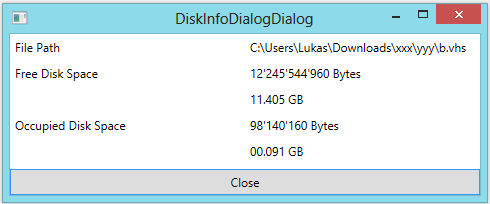
\includegraphics[scale=1]{Images/free_and_occupied_space.png} 
	\caption{Free and occupied space}
\end{figure}

% 1. Compression, if implemented with 3d party library. (1p)
\subsubsection{Compression with 3rd party library}
There are multiple compression types available. One of them is a third party implementation of the Microsoft deflate stream\footnote{http://msdn.microsoft.com/en-us/library/system.io.compression.deflatestream.aspx}.
Patterns: Decorator pattern\\
Classes: MicrosoftStreamCompressionStrategy, DeflateStream\\
Methods: DecorateToVFS, DecorateToHost\\
\begin{figure}[h!]
	\centering
	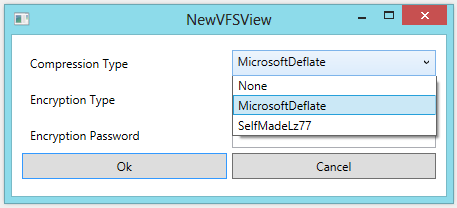
\includegraphics[scale=1]{Images/compression_types.png} 
	\caption{Compression types}
\end{figure}

% 2. Encryption, if implemented with 3d party library. (1p)
\subsubsection{Encryption with 3rd party library}
There are multiple encryption types available. One of them is a third party implementation of the Microsoft Rijndael, the AES standard\footnote{http://msdn.microsoft.com/en-us/library/system.security.cryptography.rijndael.aspx}.\\
Patterns: Decorator pattern\\
Classes:\\
Methods:
\begin{figure}[h!]
	\centering
	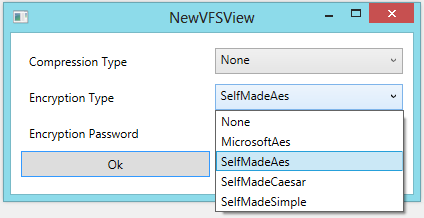
\includegraphics[scale=1]{Images/encryption_types.png} 
	\caption{Encryption types}
\end{figure}

% 3. Elastic disk: Virtual disk can dynamically grow or shrink, depending on its occupied space. (2p)
\subsubsection{Elastic disk}
The elastic disk is implemented. The file system only allocates disk space when it is required and there are no "practical" limit for the file size or the disk size. It probably will be limited either by the host file system or the hardware itself. The file system is designed in such a way that it does not need to reorganize itself to be fast (known as defragmentation).\\
Classes: BlockAllocation\\
Methods: BlockAllocation.Allocate

% 1. Compression, if implemented by hand (you can take a look at the arithmetic compression8). (2p)
\subsubsection{Compression implemented by hand}
Compression by hand is implemented. The basic idea behind the compression is the LZ77 algorithm\footnote{http://www.ieeeghn.org/wiki/index.php/Milestones:Lempel-Ziv\_Data\_Compression\_Algorithm,\_1977}.\\
Classes: SelfMadeLz77Stream, Lz77Triple, Lz77Constants, CircularBuffer, SelfMadeLz77StreamCompressionStrategy\\
Methods: SelfMadeLz77Stream.Read, SelfMadeLz77Stream.Write

% 2. Encryption, if implemented by hand. (3p)
\subsubsection{Encryption implemented by hand}
Encryption was also implemented by hand. There is a simple encryption and a caesar encryption which are fast, but very weak. Therefore, the AES-256 with CBC\footnote{part of the AES standard, http://csrc.nist.gov/publications/fips/fips197/fips-197.pdf} was implemented.\\
Classes: SelfMadeAes256Cryptor, AesHelperMethods, AesConstants\\
Methods: SelfMadeAes256Cryptor.EncryptBlocks, SelfMadeAes256Cryptor.DecryptBlocks\\


% 3. Large data: This means, that VFS core can store & operate amount of data, that can't t to PC RAM ( typically, more than 4Gb). (3p)
\subsubsection{TODO}
TODO.\\
Classes:\\
Methods:\\
\begin{figure}[h!]
	\centering
	
\includegraphics[scale=1]{Images/todo.png} 
	\caption{TODO}
\end{figure}




% 
\subsubsection{TODO}
TODO.\\
Classes:\\
Methods:\\
\begin{figure}[h!]
	\centering
	
\includegraphics[scale=1]{Images/todo.png} 
	\caption{TODO}
\end{figure}




\subsection{Design}

% TODO: Remove this text and replace it with actual content
\emph{Give an overview of the design of this part and describe in general terms how the implementation works. You can mention design patterns used, class diagrams, definition of custom file formats, network protocols, or anything else that helps understand the implementation.}

\subsection{File Format}

The design of the file format is related to the Unix File System (UFS) and the New Technology File System (NTFS). The file is partitioned into two sections (reference / citation needed):

\begin{itemize}
  \item one super block
  \item many normal blocks
\end{itemize}

\begin{figure}[h!]
  \framebox(100,20){Super block}
  \put(0,0){\framebox(290,20){Normal blocks}}
  \put(0,-20){\framebox(15,20){$b_{1}$}}
  \put(15,-20){\framebox(15,20){$b_{2}$}}
  \put(30,-20){\framebox(15,20){$b_{3}$}}
  \put(45,-20){\framebox(245,20){...}}
  \put(275,-20){\framebox(15,20){$b_{n}$}}
  \caption{Partitions of the virtual disk with $n$ normal blocks.}
\end{figure}


\subsubsection{Super Block}

The super block has a constant size of 32 KB. Although most of the space is not needed yet, it can be used to save meta information about the file system:
\begin{itemize}
  \item block amount and block size\\
  ($block\_amount * block\_size + super\_block\_size = disks\_size$)
  \item version of the file format
  \item date/time created of the virtual disk
  \item compression algorithm(s)
  \item file encryption algorithm(s)
  \item encrypted key for file encryption
  \item hashed seed/password for file encryption
  \item etc.
\end{itemize}

\subsubsection{Normal Blocks}

The normal blocks consist of many blocks of a fixed block size. The block size is stored in the file system meta information, which is stored in the super block. The block size is the same for every block and cannot be changed after creating the file. Tough it is possible to change the block amount, which is known as growing or shrinking the virtual file.

\paragraph{Normal Block Types} ~\\

\noindent One normal block can be of one of the following types:

\begin{itemize}
  \item Index Node
    \item Root Node
    \item File Node
    \item Folder Node
  \item File Content Node
  \item Indirect Node
\end{itemize}

\paragraph{Index Node} ~\\

(TODO: always use "folder" or always use "directory", TBD).

The Index Node contains the file type (file or directory, 1 byte) and the name (max. 255 bytes, can contain any character excluding '/' and '$\backslash0$') of one object. The next 64 byte contain the block count of the blocks, which are referenced  (through the Indirection Nodes) by this Index node. The next block\_reference\_size byte (usually 64 byte) contain the indirection node number, which is a reference to the indirection node. If the Index Node is a file, then the next 32 byte describe the length of the last block.\\


At the start of the normal blocks, at block $b_{0}$, there is always exactly one Root Node. The root node is a special kind of folder, but unlike the other Index Nodes, the Root Node does not have a name. Otherwise, the Root Node works exactly like a Folder Name, which is described below.\\

(Not implemented yet: The block $b_{1}$ is reserved for other meta information, also organized as a folder).\\

If and only if the file type is a directory, then the Index Node contains references to other Index Nodes (files and directories). These are considered sub-files and sub-directories. The referenced Index Nodes can be ordered by name, so searching becomes faster ($\mathcal{O}(log(n))$ instead of $\mathcal{O}(n)$). To implement this, an AVL or a B-Tree can be used. A B-Tree would be better, but an AVL tree is simpler to implement. (Currently, none of these data structures are used or implemented yet. Therefore searching currently takes $\mathcal{O}(n)$).\\

If and only if the file type is a file, then the Index Node contains references to File Content Nodes. These File Content Nodes must be accessible in the same order they were put into the file system. Because of the concept of the Indirection Nodes, random access is possible. Therefore, seeking to any block in the file takes $\mathcal{O}(1)$, which is very good, especially if only a very small part of a huge file is needed.\\

The File Content Node contains only file content. This content can be encrypted and/or compressed.\\

The Indirect Nodes are used to address multiple blocks. There are three levels of Indirect Nodes. First, the one which is referenced by the Index Node (File Node or Folder Node), is the 1st level Indirect Node. This one references to multiple 2nd level indirect nodes. Any of the 2nd level Indirect Nodes references to multiple 3rd Indirect Nodes. And every 3rd Indirect Node references to multiple blocks, which are of type Index Node. For folders, these addressed blocks are File Nodes or Folder Nodes. For files, these addressed blocks are File Content Nodes.\\

$$references\ per\ Indirect Node = \cfrac{block\ size}{block\ reference\ size}$$



(TODO: add a good figure...)\\

(TODO: After this: old, has to be adjusted)\\
\\




\paragraph{The Block Size} ~\\

\noindent Because of the type and the name ($ = 1\ byte + 255\ bytes$), the block size must be larger than 256 bytes. In general, there is no good block size tough. If very many small files are stored and the block size is chosen  large (e.g. 32 KB), then there are huge losses because of the internal fragmentation (the rest of the block is unused). If the files are very large, the overhead to manage the data is huge, especially if the block size is very small (e.g. 512 bytes). So if rather few large files are stored in the VFS, the block size should be large, and if many small files are stored, the block size should be small. A good compromise is a block size of 2-8 KB (further literature/ links / reasoning / calculations / proofs required for these statements).

\paragraph{The Block Reference Size} ~\\

\noindent The block reference size determines, how many blocks can be addressed. There are $2^{block\_reference\_size}$ blocks that can be addressed.

\subsection{Block Allocation}

In this project, the blocks are allocated from the beginning of the file system to the end of the file system. The system has a pointer to the next free block when running. If a block is used for an object, this pointer is moved to the next free block in the file system. This can end up using O(n) time to find a free block, which is suboptimal. If a block is deleted, this pointer is not moved back to the free block. This can lead to external fragmentation, but partly prevents internal fragmentation (further literature/ links / reasoning / calculations / proofs required for these statements). If the pointer points to the last block of the file system and this block is reserved, but there is still free space in the file system, the pointer is moved back to the beginning.

\subsection{Indices}

Due to the simplicity of the block allocation, there is no need to store an index of free blocks.

For the filename search, it would be convenient if the file names were stored in an ordered list. This could be achieved by storing the names in an AVL tree (citiation / source needed here). This would enable the file system to
find a file name in $\mathcal{O}(log(n))$ time instead of $\mathcal{O}(n)$. Due to the complexity, this is not implemented (yet).

\subsection{Data fragmentation}

Due to the simple block allocation strategy, data fragmentation can occur. To avoid this, there are two possibilities:

\begin{itemize}
  \item Alternate block allocation strategy to avoid data fragmentation
  \item A de-fragmentation procedure which de-fragments the data
\end{itemize}

Due to simplicity, none of these are implemented (yet).

\subsection{Growing and shrinking the disk}

As mentioned above, the disk can grow or shrink by changing the amount of blocks.

\subsubsection{Growing}

To grow the disk, additional blocks are added at the end of the disk. Additionally, the normal block amount is increased in the super block.

\subsubsection{Shrinking}

However, shrinking is more difficult, because the last block could be occupied, even if the disk is not full. Therefore, the last blocks have to be moved to free blocks, and the reference to this block has to be adjusted. This is very complex to implement efficiently and is therefore not implemented in this project (yet).\\
Additionally, the normal block amount is decreased in the super block.

\subsection{Formulas and Pseudocode}

\begin{equation}
\begin{split}
maximal\_file\_size =
  \bigg(\cfrac{block\ size}{block\ reference\ size}\bigg)^3 +\\
  \bigg(\cfrac{block\ size}{block\ reference\ size}\bigg)^2 +\\
  \bigg(\cfrac{block\ size}{block\ reference\ size}\bigg) +\\
  (n=10, TBD)) * block\ size.
\end{split}
\end{equation}

\begin{equation}
maximal\ amount\ of\ blocks = 2^{block\ reference\ size}
\end{equation}



\subsection{Fault tolerance}

No fault tolerance (e.g. on power loss) is implemented (yet). For this, journaling could be implemented.\\
\\







If the amount of directories is smaller or equal to (block\_size - 256 bytes) / block\_reference\_size, 
then all references are stored in that file. Otherwise, it works like the large files with Indirect Nodes.\\


Iff the Index Node type is file, then there are two possibilities:

\begin{enumerate}
  \item Small file content\\
  The content of the file is very small (block size minus 1 type byte and 255 name bytes) and can be stored in the index node. Then the content of the file is stored in this very Index Node.
  \item Large file content\\
The content of the file exceeds the block size (minus the type byte and the name bytes = 256 bytes).\\
Each reference to a file content block (description of file content block: see below) is of size $2^{block\_reference\_size}$, which allows maximum virtual file sizes of $2^{(block reference size, n=8, TBD)} * block\_size + super\_block\_size$.\\
\begin{enumerate}
  \item No indirection: The first (n=10, TBD) block references directly refer to file content blocks. This is (n=10, TBD) * block\_reference\_size bytes of size.
  \item Single indirection: The next "block reference" references to one indirect node, which references to ($block\_size / block\_reference\_size$) other file content blocks each.
  \item Double indirection: The next "block reference" references to one indirect node, which references to $block\_size / block\_reference\_size$ indirect nodes each, which references to $block\_size / block\_reference\_size$ other file contents each.
  \item Triple indirection: The next "block reference" references to one indirect node, which references to $block\_size / block\_reference\_size$ indirect nodes each, which reference to $block\_size / block\_reference\_size$ indirect nodes each, which references to $block\_size / block\_reference\_size$ other file contents each.
\end{enumerate}
\end{enumerate}

TODO: add reference to formulas\\

\end{document}


% PART II: VFS Browser
% --------------------------------------

\section{VFS Browser}

% TODO: Remove this line
\textbf{[This section has to be completed by April 22nd.]}

%TODO: Remove this text and replace it with actual content
\emph{Give a short (1-2 paragraphs) description of what VFS Browser is.}


\subsection{Requirements}

% TODO: Remove this text and replace it with actual content
\emph{Describe which requirements (and possibly bonus requirements) you have implemented in this part. Give a quick description (1-2 sentences) of each requirement. List the software elements (classes and or functions) that are mainly involved in implementing each requirement.}


\subsection{Design}

% TODO: Remove this text and replace it with actual content
\emph{Give an overview of the design of this part and describe in general terms how the implementation works. You can mention design patterns used, class diagrams, definition of custom file formats, network protocols, or anything else that helps understand the implementation.}


\subsection{Integration}

% TODO: Remove this text and replace it with actual content
\emph{If you had to change the design or API of the previous part, describe the changes and the reasons for each change here.}



% PART III: Synchronization Server
% --------------------------------------

\section{Synchronization Server}

\documentclass[JCDReport.tex]{subfiles} 
\begin{document}

The synchronization server propagates changes from one machine to another using a network connection. The management of the distributed VFSs is made on an account basis, i.e. in order to use the server, a user must have an account and link a virtual disk to this account. Therefore the server allows user to register and login after successful registration. Once the user enters the online mode (see GUI part) the currently open disk is synchronized to the server automatically. After initial synchronization, every synchronized disk gets a unique ID, so the disk can be identified. A user can have multiple disks, while a disk belongs to a single user. Unlinked disks are not synchronized. There is an automatic conflict recognition so the user can resolve conflicts by rolling back to a specific version, which is not conflicted, and then restart the synchronization again.\\

Technically the server is implemented as a WCF \footnote{http://msdn.microsoft.com/en-us/library/dd456779.aspx} service  and it allows multiple parallel connections. A an optional requirement, automatic persistence was implemented using SQLite. The usage of SQLite for this optional requirement was allowed by Alexey Kolesnichenko \footnote{https://piazza.com/class\#spring2013/252028400l/41}.\\

\subsection{Requirements}

% TODO: Remove this text and replace it with actual content
\emph{Describe which requirements (and possibly bonus requirements) you have implemented in this part. Give a quick description (1-2 sentences) of each requirement. List the software elements (classes and or functions) that are mainly involved in implementing each requirement.}


% 1. The browser should allow the user to create a new account or to log in to an existing account.
\subsubsection{Registration and login}
There are two forms for registration and login.\\
Classes: MainViewModel, DiskServiceClient\\
Commands: LoginCommand, LogoutCommand

\begin{figure}[h!]
	\centering
	\begin{subfigure}[b]{1\textwidth}
		\centering
		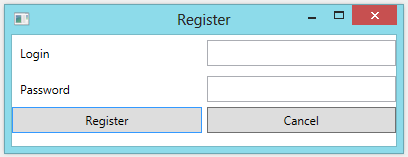
\includegraphics[scale=1]{Images/registration.png}
		\caption{Registration functionality}
	\end{subfigure}
	
	\begin{subfigure}[b]{1\textwidth}
		\centering
		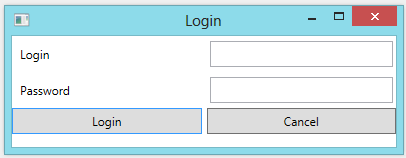
\includegraphics[scale=1]{Images/login.png} 
		\caption{Login functionality}
	\end{subfigure}
	\caption{Registration and login}
\end{figure}

% 2. The browser should offer to switch to an offine mode, and be able to operate without a connection to the server.
\subsubsection{Online / offline mode}
The user can switch between online and offline mode.\\
Classes: MainViewModel, DiskServiceClient, SynchronizationViewModel, SynchronizationService\\
Commands: SwitchToOnlineModeCommand, SwitchToOfflineModeCommand
\begin{figure}[h!]
	\centering
	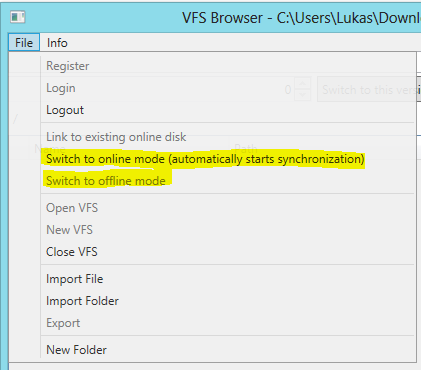
\includegraphics[scale=1]{Images/onlineofflinemode.png} 
	\caption{Online and offline switch}
\end{figure}	

% 3. The browser should support binding an existing virtual disk to an active account.
\subsubsection{Binding of existing disk}
The user can bind an existing disk to the local machine. Synchronization will then start automatically.\\
Classes: MainViewModel, DiskBrowserViewModel, DiskServiceClient\\
Commands: LinkDiskCommand
\begin{figure}[h!]
	\centering
	
\includegraphics[scale=1]{Images/todo.png} 
	\caption{Binding an existing virtual disk}
\end{figure}	

% 1. The server should support registration of unique accounts. Each account includes name & password.
\subsubsection{Registration of unique accounts}
The server provides a registration of unique user accounts. Each account includes name and password. To make registered users persistent, SQLite is used. If persistence would not have been implemented, a dictionary with the login as key could have been used.\\
Classes: UserDto, DiskServiceImpl, PersistenceImpl
\begin{figure}[h!]
	\centering
	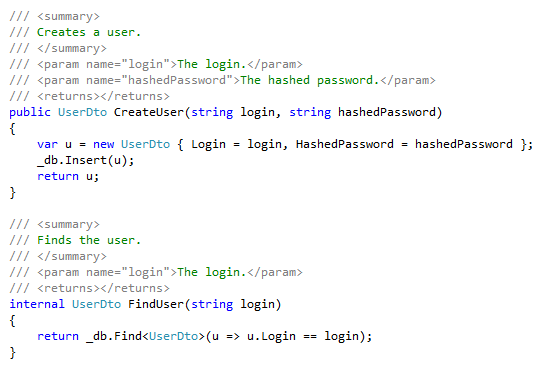
\includegraphics[scale=1]{Images/login_server.png} 
	\caption{Code to persist and to find a user}
\end{figure}


% 2. The server should track changes to linked virtual disks of registered accounts and synchronize the changes across the machines.
\subsubsection{Atuomatic synchronization across machines}
Once a disk is bound to a server and the client is in online mode, the local changes are synchronized across the machines automatically. If remote changes occur, the client automatically downloads all changes from the server.
\begin{figure}[h!]
	\centering
	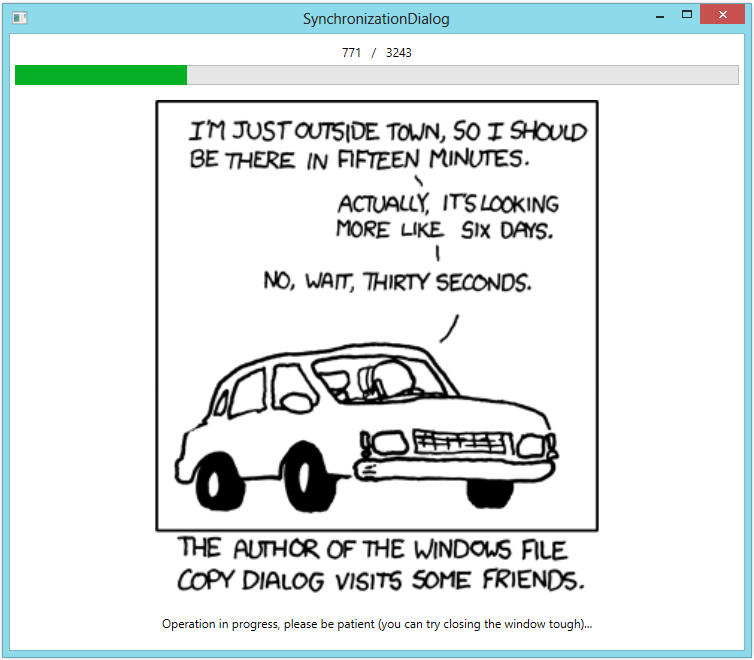
\includegraphics[scale=0.7]{Images/synchronization_dialog.png} 
	\caption{The synchronization dialogue}
\end{figure}

% 1. Provide a set of mocked unit tests for your implemenation.
\subsubsection{Mocked unit tests}
Because of the IoC pattern, mocked unit tests are fairly easy to implement. For example, in the VFSConsoleTests project, the FileSystemTextManipulatorMock mocks the FileSystemTextManipulator. Therefore the console can be tested without the FileSystemTextManipulator. Additionally, there are InOutMocks to mock the input / output.
\begin{figure}[h!]
	\centering
	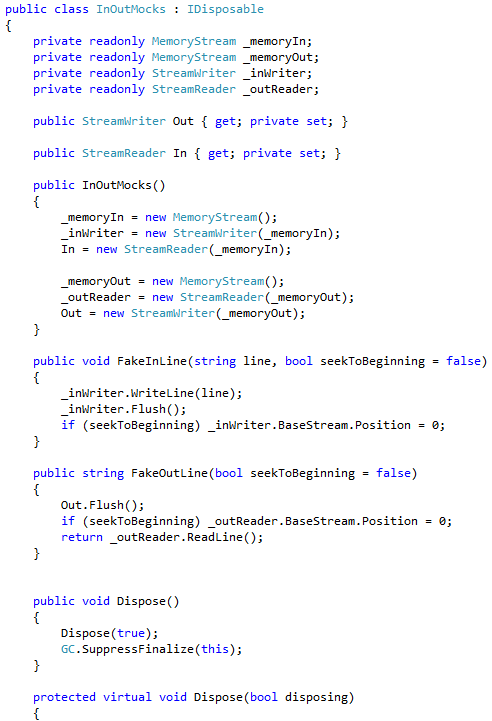
\includegraphics[scale=1]{Images/inoutmocks.png} 
	\caption{The input / output mocks to test the console application}
\end{figure}

% 2. Conflict Resolution: implement a conflict resolution scheme, so that concurrent changes to the same file are not lost (e.g. saving conflicting files as separate versions).
\subsubsection{Conflict resolution}
There is an automatic conflict recognition so the user can resolve conflicts by rolling back to a specific version, which is not conflicted, and then restart the synchronization again.\\
While the file system is conflicted, read operations are still possible. This way, the user can export a file he changed, roll back to a older version, synchronize the disk, and then import the file he changed again.
\begin{figure}[h!]
	\centering
	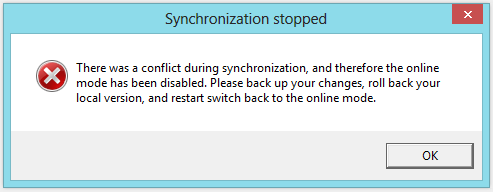
\includegraphics[scale=1]{Images/synchronization_conflict1.png}
	\caption{Conflict recognition}
\end{figure}
\begin{figure}[h!]
	\centering
	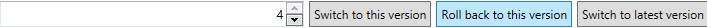
\includegraphics[scale=0.75]{Images/synchronization_conflict2.png}
	\caption{Conflict resolution}
\end{figure}

% 1. The browser is updating automatically when changes to the disk occur.
\subsubsection{Automatic updates}
The browser is updating automatically when changes to the disk occur. To make this possible, the file system provides an event, which fires when changes to the file system occur. The GUI registers to this event. This is the .NET / WPF implementation which is very similar to the observer pattern.\\
Classes: FileSystem, FileSystemTextManipulator, MainViewModel\\
Events: FileSystemChanged
\begin{figure}[h!]
	\centering
	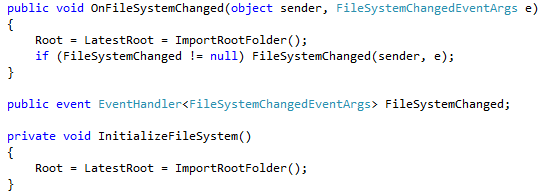
\includegraphics[scale=1]{Images/file_system_changed1.png} 
	\caption{Automatic updates: the event implementation in the file system class}
\end{figure}
\begin{figure}[h!]
	\centering
	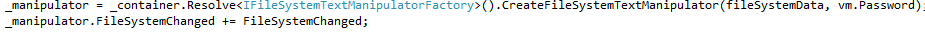
\includegraphics[scale=1]{Images/file_system_changed2.png} 
	\caption{Automatic updates: the MainViewModel registers to updates when the file system is changed}
\end{figure}
\begin{figure}[h!]
	\centering
	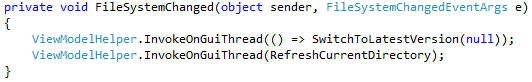
\includegraphics[scale=1]{Images/file_system_changed3.png} 
	\caption{Automatic updates: Is executed when the file system is changed.}
\end{figure}


% 2. The server is able to synchronize changes, which are done simultaneously on the same account on different machines.
\subsubsection{Simultaneous synchronization}
The server is implemented as a WCF \footnote{http://msdn.microsoft.com/en-us/library/dd456779.aspx} service  and it allows multiple parallel connections.\\
For every new connection, a new IDiskService is instantiated. This allows multiple connections to the server and thus parallel synchronization of changes.\\
Classes: IDiskService, DiskServiceImpl, ServiceContract
\begin{figure}[h!]
	\centering
	
\includegraphics[scale=1]{Images/todo.png} 
	\caption{TODO}
\end{figure}

% Incremental Changes: minimize the communication between the browser and the server by only transfering the parts of a file that changed.
\subsubsection{Incremental changes}
The synchronization only requires to synchronize the blocks which have not been synchronized before.\\
For this, the DiskDto (persisted on the server) stores the NewestBlock which is to synchronize. Locally, every file system stores the blocks used in the root folder (BlocksUsed property) of the current version. When the synchronization starts, only $$Math.abs(NewestBlock_{OnServer}-BlocksUsed_{Locally})$$ have to be synchronized.\\
Classes: SynchronizationService
\begin{figure}[h!]
	\centering 
	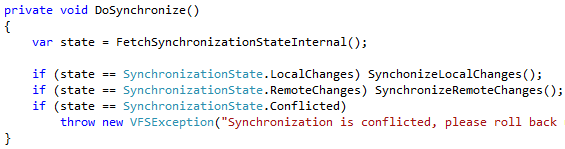
\includegraphics[scale=1]{Images/do_synchronization.png} 
	\caption{Incremental changes: synchronize remote changes or local changes}
\end{figure}
\begin{figure}[h!]
	\centering 
	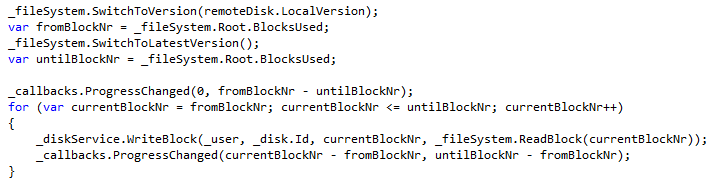
\includegraphics[scale=1]{Images/incremental_changes.png}
	\caption{Incremental changes: only synchronize blocks which have not been synchronized yet}
\end{figure}

% 3. File History: provide a history for les and an interface to restore a previous version.
\subsubsection{File history}
There is a file history available. The user can switch to an older version and export files from there, and he also can roll back to an older version, discarding all changes in later versions.\\
Technically, the file history is implemented like this:\\
In the beginning, there is one root node. Every change in the file system then leads to a new root node, which points back to the old root node. The new root node contains block references to all children of the old root node which have not been changed during the update of the file system. Additionally, the new root node contains references to the newly created nodes. So, for every version of the history, a new root node is created. The file system options, which are stored at the start of the file system, point to the latest root node in the file system.\\
\emph{
Example: Given the $root folder_{v1}$ contains a $folder a_{v1}$ and $b_{v1}$. $folder a_{v1}$ also contains a subfolder $folder x_{v1}$. The options point to the $root folder_{v1}$.\\
Now a new subfolder $y_{v2}$ should be created within the folder $a_{v1}$.\\
Then a new folder $a_{v2}$ is created, which references to the new subfolder $y_{v2}$ and to the old folder $folder a_{v1}$. Next, a new $root folder_{v2}$ is created. It creates a back link to $root folder_{v1}$, so it can switch back to an older version. Additionally, the new $root folder_{v2}$ contains a reference to the folder $b_{v1}$ (old reference) and a reference to $a_{v2}$ (new reference). After this, the options now point to the $root folder_{v2}$.\\
}\\
This gives us multiple advantages: Firstly, a written block never will change again (immutable object pattern). Therefore, synchronization is faster, because only the newly created blocks have to be synchronized. Furthermore, copy operations do not depend on the file size or the amount to copy. Thus the time to copy only depends on the length of the path of the files to copy.\\
Classes: FileSystem, BlockList\\
Methods: FileSystem.ArchiveAndReplaceRoot, BlockList.CopyReplacingReference

\begin{figure}[h!]
	\begin{subfigure}[b]{1\textwidth}
		\centering
		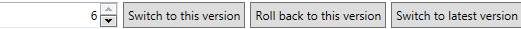
\includegraphics[scale=1]{Images/history.png}
		\caption{The file history GUI}
	\end{subfigure}
	
	\begin{subfigure}[b]{1\textwidth}
		\centering
		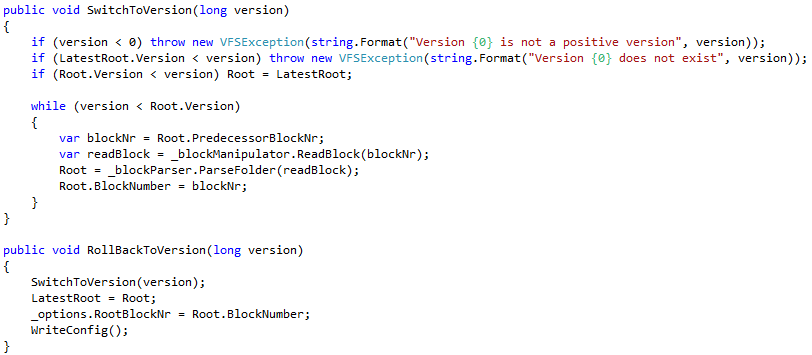
\includegraphics[scale=0.5]{Images/history_implementation.png}
		\caption{The file history implementation (FileSystem)}
	\end{subfigure}
	
	\begin{subfigure}[b]{1\textwidth}
		\centering
		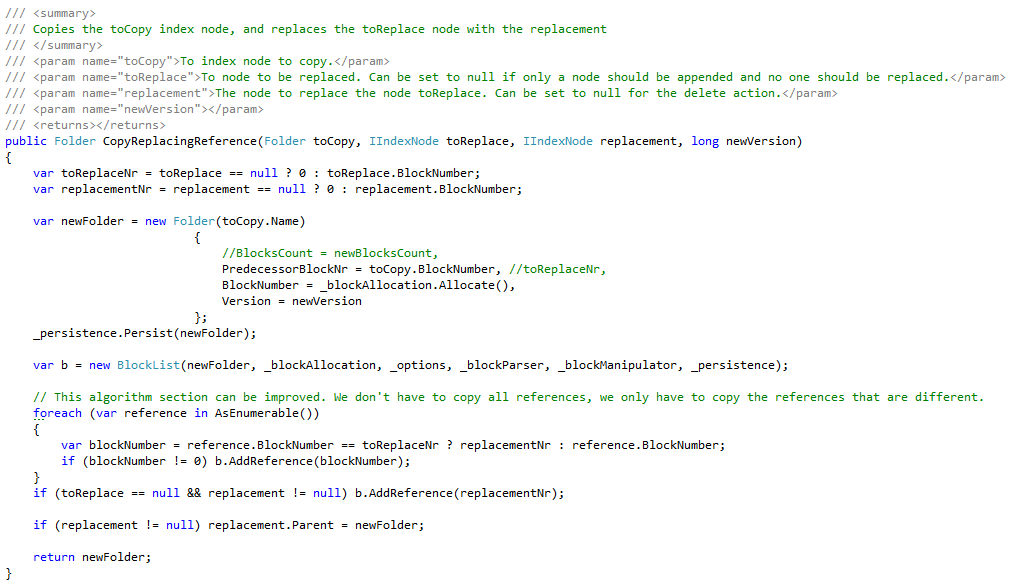
\includegraphics[scale=0.5]{Images/history_copy_replacing_reference.png}
		\caption{The file history implementation (BlockList.CopyReplacingReference)}
	\end{subfigure}
	\caption{File history}
\end{figure}


\subsection{Design}

% TODO: Remove this text and replace it with actual content
\emph{Give an overview of the design of this part and describe in general terms how the implementation works. You can mention design patterns used, class diagrams, definition of custom file formats, network protocols, or anything else that helps understand the implementation.}


\subsection{Integration}

% If you had to change the design or API of the previous part, describe the changes and the reasons for each change here.

Most of the existing design / API did not change, but it had to be enhanced for the server synchronization part. Especially, the FileSystemManipulator and the FileSystem now had to be thread safe, because the synchronization can run in the background.\\

Additionally, some existing functionality was replaced / dropped because of the history functionality and the immutable blocks. For example, the free memory command is not necessary because with the history, there is no scenario where memory is freed.\\

One very good thing were the tests. They only changed very little since they were written, and they provided immediate feedback, if something went wrong during a refactoring or by enhancing the system. The also run very fast and are run parallel by the Visual Studio 2012.

\end{document}
















% PART IV: Quick Start Guide
% --------------------------------------

\section{Quick Start Guide}

\documentclass[JCDReport.tex]{subfiles} 
\begin{document}

\subsection{Installation}

Fist, install the Git client of your preference \footnote{e.g. https://code.google.com/p/msysgit/}.\\

Then, start the command line, navigate to the folder where you would like to checkout the repository, and enter:\\
\textit{git clone git://github.com/lukaselmer/VFSPrototype.git}\\
Now, there should be a directory VFSPrototype. In the further installation instructions, the path to this folder will be referenced as \textit{repository checkout location}.\\

Before the project can be started, the following software has to be installed. Even tough the software could run on other configurations too, there is no guarantee that the software will run (correctly) with a different configuration.

\begin{enumerate}
\item Windows 8 Professional, 64 Bit
\item Visual Studio 2012 Ultimate Edition (VS2012)
\item NuGet packet manager addon\footnote{http://visualstudiogallery.msdn.microsoft.com/27077b70-9dad-4c64-adcf-c7cf6bc9970c} for VS2012 (restart VS2012 after installing the addon)
\end{enumerate}

Additionally, it is required to add the folder that contains sqlite.dll to the system path. This folder is (relative to the Git repository root): "\textit{repository checkout location}/Code/VFSPrototype/sqlite/". After this, \textbf{your pc has to be restarted}, otherwise it will probably not work.\\
In case you would not like to add this directory to the system path, you can copy the sqlite.dll and the sqlite.def to the Windows/System32 directory.\\

Then, after installing the sqlite.dll and the NuGet packet manager addon, open the solution at "\textit{repository checkout location}/Code/VFSPrototype/VFSPrototype.sln". After the project is loaded, right click on the solution and click on "Enable NuGet Package Restore", see Figure \ref{fig:nugetPackageRestore} on page \pageref{fig:nugetPackageRestore}. If this button is not available, then the NuGet package manager probably is not installed correctly.\\

\begin{figure}[h!]
	\centering
	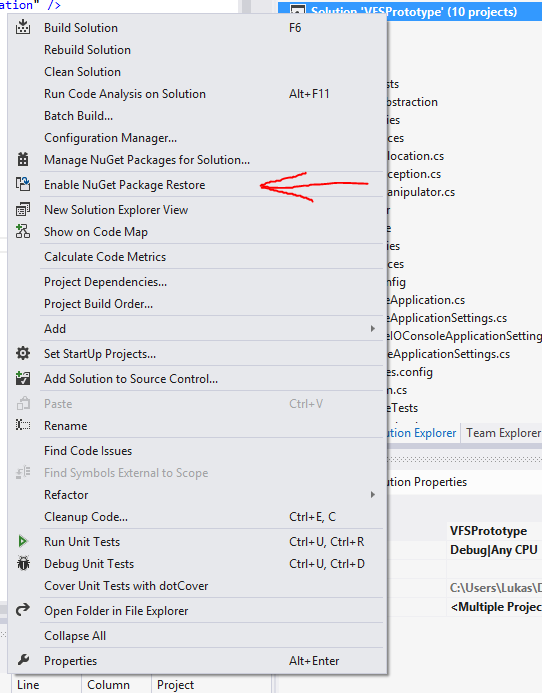
\includegraphics[scale=1]{Images/nuget_restore.png} 
	\caption{EnableNuGet Package Restore}
	\label{fig:nugetPackageRestore}
\end{figure}	

To start the server, right click on the project "VFSWCFContracts", click "Debug"/"Start new instance". Now the server should be running and a new browser window should open.\\

To start the client, right click on the project "Startup", click "Debug"/"Start new instance". Now the client should be running and a new window with the file system browser should open.\\

You can start as many clients a you would like.\\

There is one more catch, literally. Try the login functionality with some wrong credentials. Now the VS2012 will witch to the debug mode, because a FaultException was thrown. This is inconvenient, because these exceptions are propagated to the client, because of the FaultContracts. To disable this behaviour, stop the program, and click on "Debug"/"Exceptions" in the VS2012 main menu bar. Then a new window should occur. Click on "Find..." and enter "FaultException". You should find two items "FaultException" and "FaultException'1". Disable all flags of these two exceptions, especially the "User-unhandled" checkbox. Press ok, and you will not see this exception again.


\subsection{Console Application}

% If you have a command line interface for your VFS, describe here the commands available (e.g. ls, copy, import).

The console application was developed at the beginning of the project. Therefore, many options available in the GUI are not available in the console.\\

Available commands:
\begin{itemize}
\item cd
\item delete
\item exists
\item exit
\item export
\item help
\item import
\item ls
\item mkdir
\end{itemize}



\subsection{Scenario}

% TODO: Remove this text and replace it with actual content
% Describe how to realize the following use case with your system. Describe the steps involved and how to perform each action (e.g. command line executions and arguments, menu entries, keyboard shortcuts, screenshots). The use case is the following:
%\begin{enumerate}
%\item Start synchronization server on localhost.
%\item Create account on synchronization server.
%\item Create two VFS disks (on the same machine) and link them to the new account.
%\item Import a directory (recursively) from the host file system into Disk 1.
%\item Dispose Disk 1 after the synchronization finished.
%\item Export the directory (recursively) from Disk 2 into the host file system.
%\item Stop synchronization server.
%\end{enumerate}
%}


\begin{figure}[h!]
	\centering
	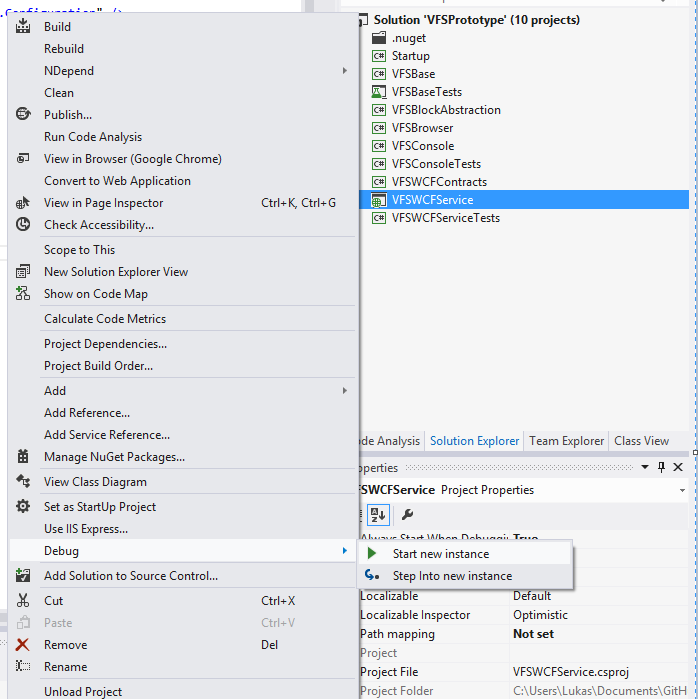
\includegraphics[scale=0.75]{Images/tutorial/1.png} 
	\caption{synchronization server on localhost.}
\end{figure}	

\begin{figure}[h!]
	\centering
	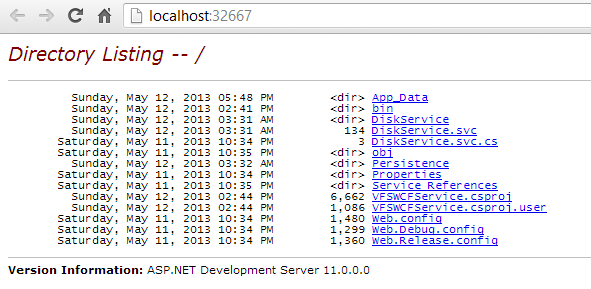
\includegraphics[scale=0.75]{Images/tutorial/2.png} 
	\caption{You should see this.}
\end{figure}

\begin{figure}[h!]
	\centering
	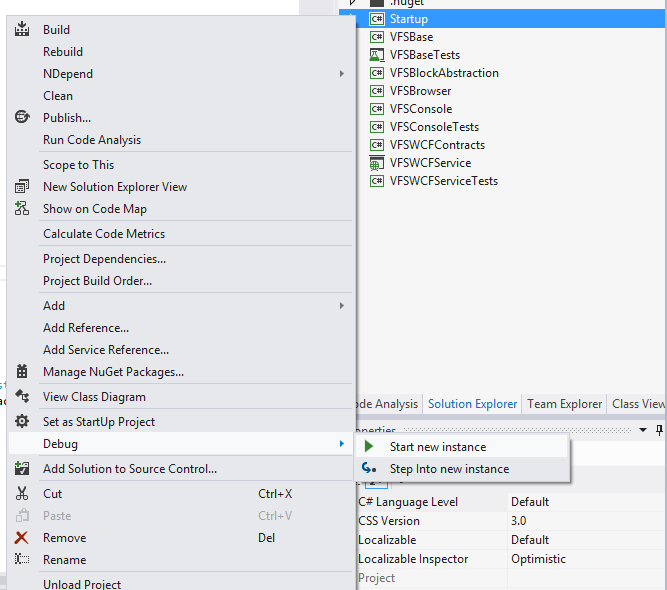
\includegraphics[scale=0.75]{Images/tutorial/3.png} 
	\caption{Start the client (do this two times to start two clients).}
\end{figure}

\begin{figure}[h!]
	\centering
	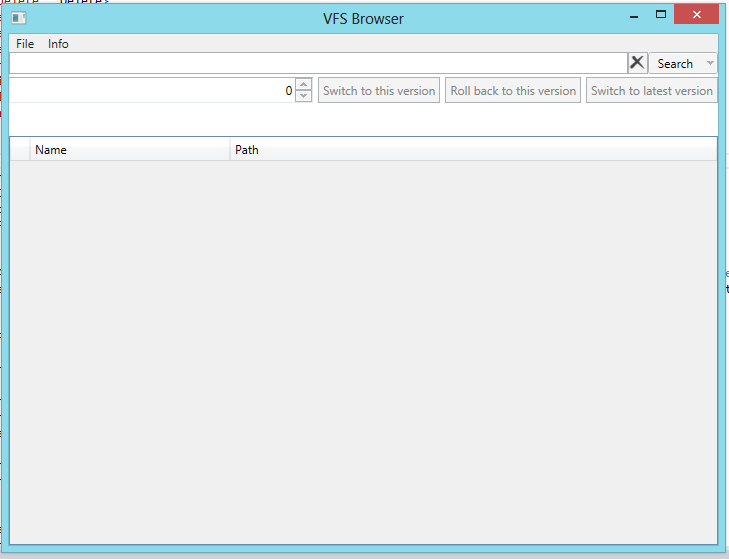
\includegraphics[scale=0.75]{Images/tutorial/4.png} 
	\caption{You should see this (two times if the client has been started two times).}
\end{figure}

\begin{figure}[h!]
	\centering
	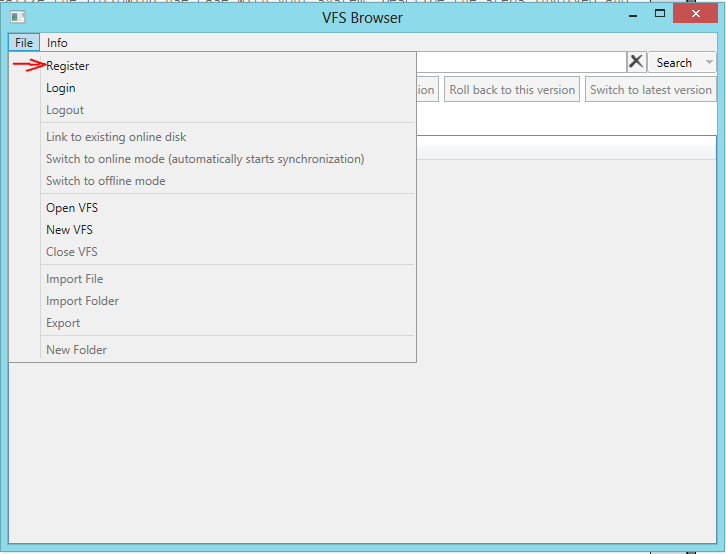
\includegraphics[scale=0.75]{Images/tutorial/5.png} 
	\caption{Register a new user account.}
\end{figure}

\begin{figure}[h!]
	\centering
	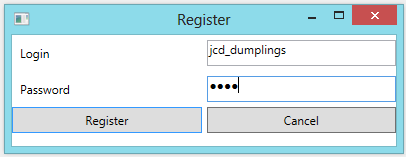
\includegraphics[scale=1]{Images/tutorial/6.png} 
	\caption{Enter credentials.}
\end{figure}

\begin{figure}[h!]
	\centering
	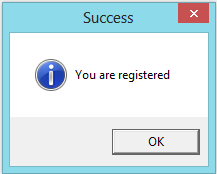
\includegraphics[scale=1]{Images/tutorial/7.png} 
	\caption{Registration successful.}
\end{figure}

\begin{figure}[h!]
	\centering
	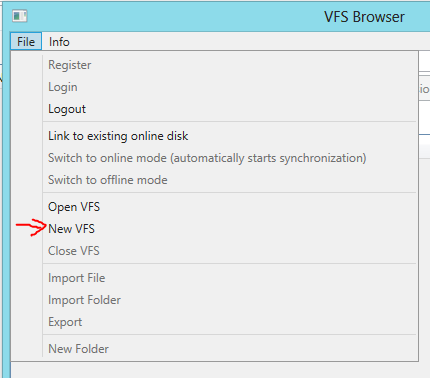
\includegraphics[scale=1]{Images/tutorial/8.png} 
	\caption{Create a new (local) VFS.}
\end{figure}

\begin{figure}[h!]
	\centering
	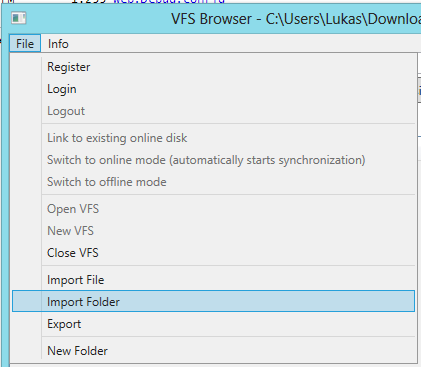
\includegraphics[scale=1]{Images/tutorial/8_2.png} 
	\caption{Import any folder.}
\end{figure}

\begin{figure}[h!]
	\centering
	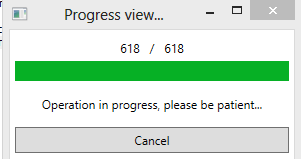
\includegraphics[scale=1]{Images/tutorial/9.png} 
	\caption{You should see the progress bar from the import.}
\end{figure}

\begin{figure}[h!]
	\centering
	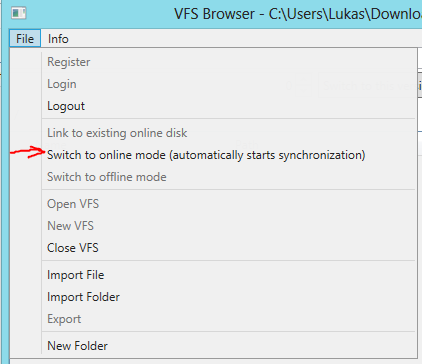
\includegraphics[scale=1]{Images/tutorial/10.png} 
	\caption{Switch to online mode to start synchronization.}
\end{figure}

\begin{figure}[h!]
	\centering
	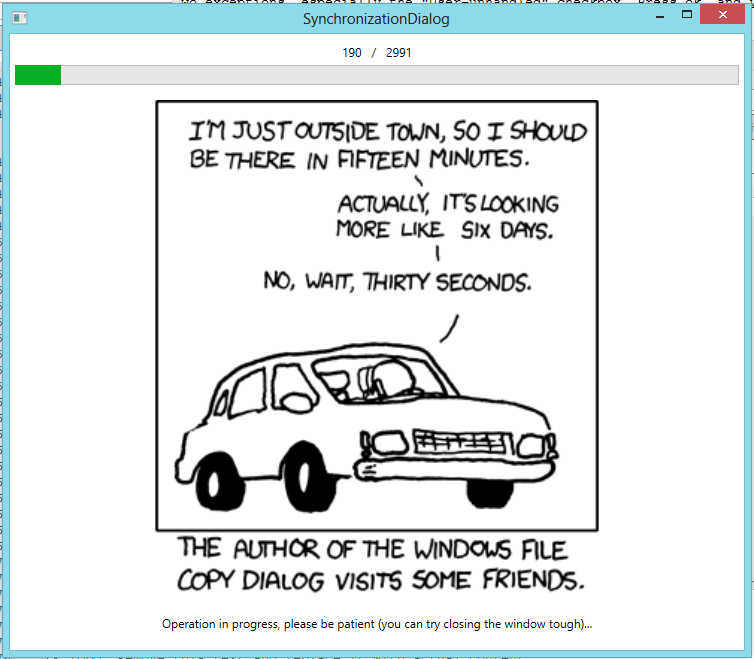
\includegraphics[scale=0.75]{Images/tutorial/11.png} 
	\caption{When the synchronization starts, you should see this dialogue.}
\end{figure}

\begin{figure}[h!]
	\centering
	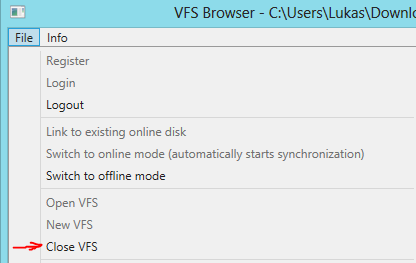
\includegraphics[scale=1]{Images/tutorial/15.png} 
	\caption{Close the VFS.}
\end{figure}

\begin{figure}[h!]
	\centering
	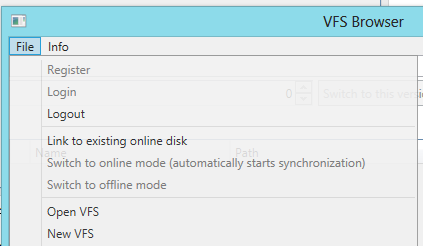
\includegraphics[scale=1]{Images/tutorial/12.png} 
	\caption{Switch to the other client, login with your credentials, and choose Link to existing disk.}
\end{figure}

\begin{figure}[h!]
	\centering
	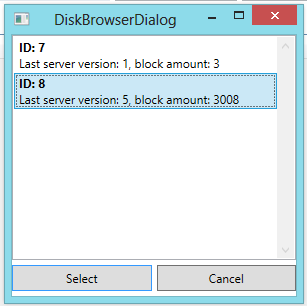
\includegraphics[scale=1]{Images/tutorial/13.png} 
	\caption{Select a disk.}
\end{figure}

\begin{figure}[h!]
	\centering
	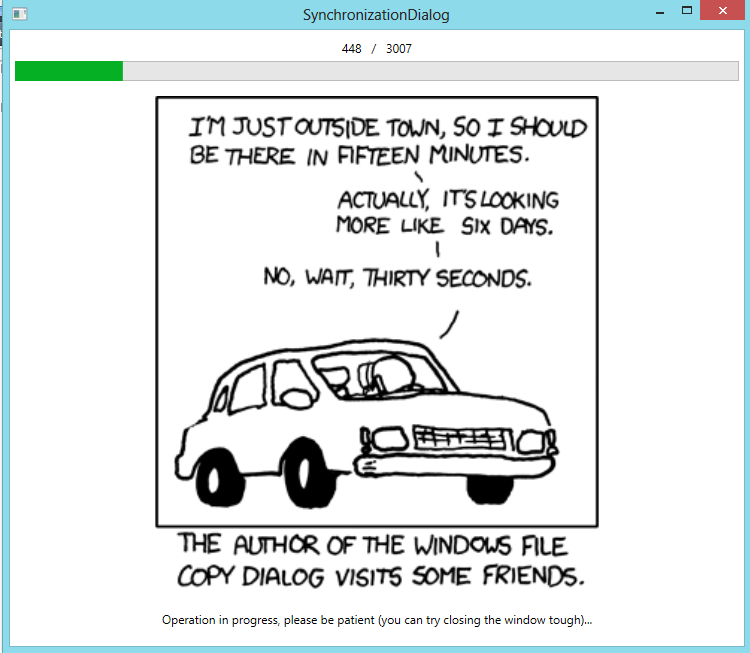
\includegraphics[scale=0.75]{Images/tutorial/14.png} 
	\caption{When switching to online mode again, you should see the synchronization dialogue.}
\end{figure}

\begin{figure}[h!]
	\centering
	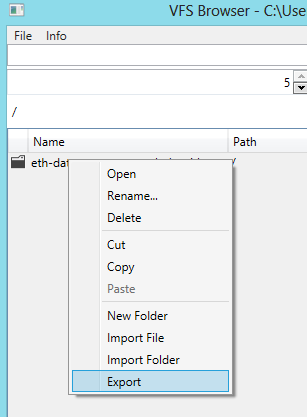
\includegraphics[scale=1]{Images/tutorial/16.png} 
	\caption{As soon as the dialogue is closed, right click on the synchronized folder to export it.}
\end{figure}

\begin{figure}[h!]
	\centering
	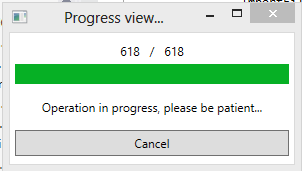
\includegraphics[scale=1]{Images/tutorial/17.png} 
	\caption{Once again, a progress report shows the export progress. After the export has finished, the folder you imported now is on the host system.}
\end{figure}



\end{document}



\end{document}
